\chapter{Marc teòric}
\label{chap:pw}
%Petita introducció tractant de justificar el nostre projecte d'una forma argumentada.  
Abans d'entrar en els detalls tècnics de la implementació i funcionament d'un BMS cal conèixer el camp en qüestió. Donat que estem parlant d'un sector en evolució i on el seu mercat està en creixement, s'ha plantejat de forma hipotètica el contrast del nostre BMS i Driver amb els del mercat per tal de poder donar-li un valor afegit. 

S'ha fet una cerca del mercat relacionat amb els vehicles elèctrics tot buscant els aspectes que donarien viabilitat a aquest projecte tractant-lo com a producte. A més a més s'ha volgut estudiar el mercat dels VE per poder visualitzar el valor que pot tenir documentar-se en aquest tema, ja que futurament els vehicles elèctrics acabaran tenint un pes molt important, ja que la tecnologia cada dia avança més i més i tots els indicis ens indiquen que el futur seran els vehicles elèctrics.
En aquest apartat es veurà l'impacte en el mercat dels vehicles elèctrics i la viabilitat que tindria la realització del projecte en comparació amb la compra directa d'un. Cal dir que donat que el treball ha estat realitzat conjuntament amb el Marc Brunet Preses, aquesta part pot ser molt similar a la seva a nivell de documentació, ja que s'ha realitzat l'estat de l'art de forma conjunta.

\section{Mercat dels cotxes elèctrics}

% El petroli, un combustible fòssil finit
A l'actualitat, l'ecologisme i l'ús d'energies sostenibles és cada cop més intens. Això ens indica que energies com l'electricitat estan agafant dia a dia una major força i per tant, tot apunta a ser un mercat que està en ple creixement. No obstant a l'actualitat, el combustible més emprat per transmetre energia a un vehicle s'extreu del petroli. El petroli és un combustible fòssil finit, i per tant, ja hi ha gent que està tenint en compte que el petroli a la llarga s'acabarà, deixant a un costat les qüestions dels efectes contaminants que es produeixen en la combustió d'aquest, ja que a nivell econòmic no és un aspecte que es tingui molt en compte. A més a més, les noves tecnologies acompanyen molt millor als vehicles elèctrics i ho faran encara més quan s'estableixin infraestructures per a carregar-los. 

Durant aquest procés d'esgotament el preu del petroli ha d'augmentar, ja que si la demanda és molt alta i la quantitat que n'existeix és molt reduïda el seu cost per força ha d'incrementar. És per això que l'impacte de vehicles elèctrics comença el seu camí per a instal·lar-se dins del mercat, ja que fa relativament poc que els vehicles elèctrics es comencen a conèixer i a manufacturar a gran escala. A més a més ja comencen a aparèixer infraestructures per a carregar aquests tipus de vehicles a les grans ciutats i per tant ja comencen a haver-hi facilitats. 
\newline
No obstant, el fet de que el petroli sigui finit no vol dir que en qüestió de 5 anys ja s'hauran esgotat totes les reserves de petroli del món, encara queden grans reserves de petroli per tot el món i les que encara no han estat trobades. La demanda del petroli segueix en augment ja que la quantitat de cotxes segueix en augment. En la següent gràfica es pot apreciar com fins l'any 2016 no ha parat de créixer la demanda del petroli:
\bigskip

% Demanda mundial de petroli, Milions de barrils per dia, valor mig per any.
\begin{figure}[H]
		\centering
    	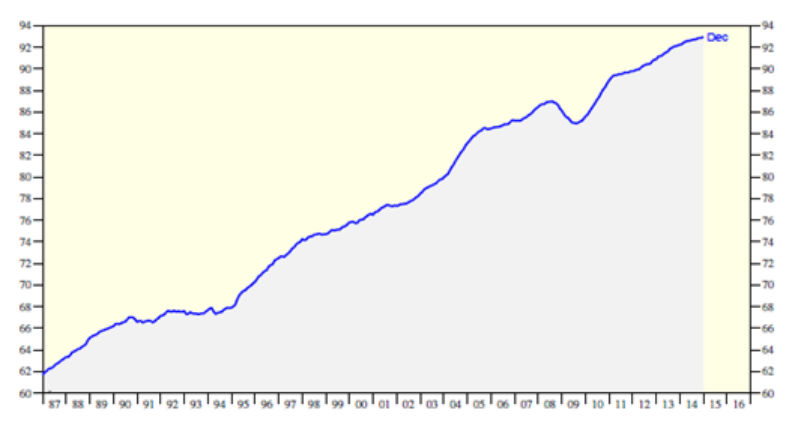
\includegraphics[width=\textwidth]{Marcteoric/Augmentdemandapetroli.png}
     	\caption{Demanda mundial de petroli, valor mig per any}
\end{figure}

\newpage

% Demanda de cotxes elèctrics al mercat
En les grans ciutats ja comencen a aparèixer polítiques que prohibeixen l'entrada a vehicles que superen un cert grau de contaminació, ja que l'acumulació d'aquest pot pujar els nivells de contaminació de la ciutat per sobre del que regeix la llei. Els vehicles elèctrics no contaminen \newline pràcticament res, si no tenim en compte el seu procés de fabricació. Els vehicles híbrids funcionen amb electricitat fins que el motor ja ha de donar una certa potència, això ja suposa que el vehicle ha d'anar a una gran velocitat, fora de les velocitats màximes permeses en una zona urbanitzada. A més a més, el preu de la gasolina és molt elevat comparat amb el de l'electricitat. 

El preu d'un vehicle de combustió o un vehicle que funciona amb electricitat no és tant distant, no estem parlant que un cotxe elèctric pugui arribar a costar el doble d'un de gasolina, els preus es troben bastant parells, tot i que encara són més econòmics els de combustió. Es preveu que per al 2022 el cost total sense subsidi per als propietaris de bateria caurà per sota de la d'un vehicle de combustió. 

Per tots aquests motius i els preus assequibles dels vehicles elèctrics, el mercat dels VE es troba en augment. La previsió per als següents anys és que la demanda creixerà de forma exponencial. Al 2040 es preveu que els vehicles elèctrics seran un 35\% de les ventes mundials d'automòbils.

\begin{figure}[H]
		\centering
    	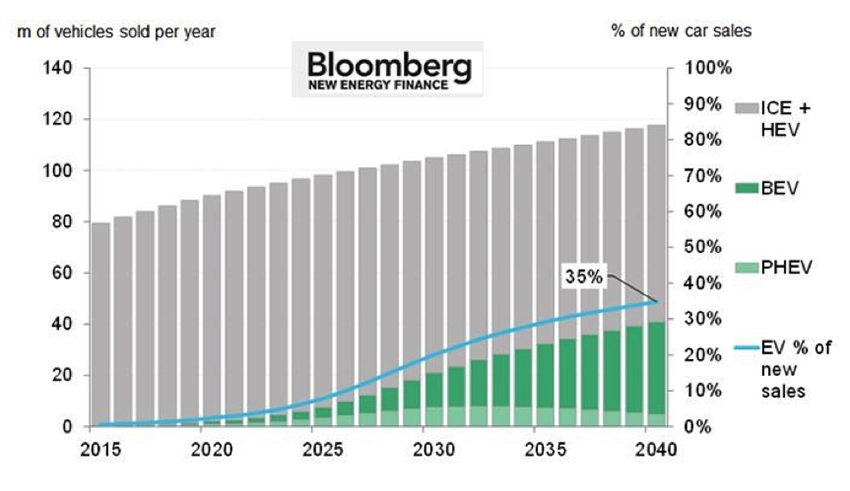
\includegraphics[width=\textwidth]{Marcteoric/ev-sales-distrib.png}
     	\caption{Previsió d'increment de la venda de vehicles elèctrics.}
\end{figure}

A la figura 2.2 es mostra de forma detallada la previsió de l'evolució del mercat dels vehicles. En primer lloc tindríem els ICE + HEV, aquests vindrien a ser els vehicles que funcionen per combustió (dièsel/gasolina) i els híbrids que també fan servir la combustió. Es pot veure com són els que lideren encara el mercat, tot indicant que el petroli seguirà sent la font d'energia principal per als vehicles en general. 

En segon lloc tindríem els BEV(Battery Electric Vehicle) que són els vehicles que funcionen mitjançant bateries. Aquests assoliran un \newline 30\% d'increment l'any 2040.Per qüestions ecològiques que podrien succeir en el futur aquest valor pot decréixer considerablement si s'estableixen límits de contaminació molt baixos. Les subvencions de l'estat per als vehicles elèctrics també podria girar la balança i que agafessin en el futur un major pes.
 

En última instància hi ha els PHEV ( Plug-In Hybrid Electric Vechicle) que són els vehicles híbrids endollables a la corrent. Encara és incert el futur d'aquest tipus de vehicles i per això no hi ha gran confiança en aquests.

\section{Mercat dels vehicles elèctrics (no cotxes)}

% Introducció
Tot i que el món dels vehicles elèctrics està totalment centrat en els cotxes, també existeixen altres vehicles que fan servir l'electricitat com a font \newline d'energia. El controlador que es plantejarà en tot aquest projecte està pensat molt més per a aquest tipus de vehicles que no pas per a cotxes. Entre aquests vehicles podríem trobar el patinet elèctric, Hoverboard i la bicicleta elèctrica entre d'altres. No només això si no que també el nostre controlador pot estar emprat per a vehicles dedicats a persones amb mobilitat reduïda com podria ser una cadira de rodes elèctrica o els típics "tricicles" que fa servir la gent gran. Per últim caldria posar els vehicles radiocontrol(RC), des de llanxes fins avions. 

Per a la majoria de vehicles esmentats no és precís aconseguir carnet de conduir o bé una llicència ni assegurança, però ve cal conèixer la normativa que regula l'ús d'aquests vehicles en llocs urbans. Cada municipi té els seus permisos i prohibicions. La normativa pot canviar depenent del pes o bé la velocitat màxima. Per això s'aconsella informar-se sobre la legislació del seu ajuntament. Sobretot a les grans ciutats és on la legislació és més estricta. Un exemple d'aquest podria ser la legislació actual de Barcelona sobre els patinets elèctrics. Els patinets elèctrics conformen els vehicles elèctrics de Tipus B.

% Normativa de patinets elèctrics a Barcelona
\begin{figure}[H]
		\centering
    	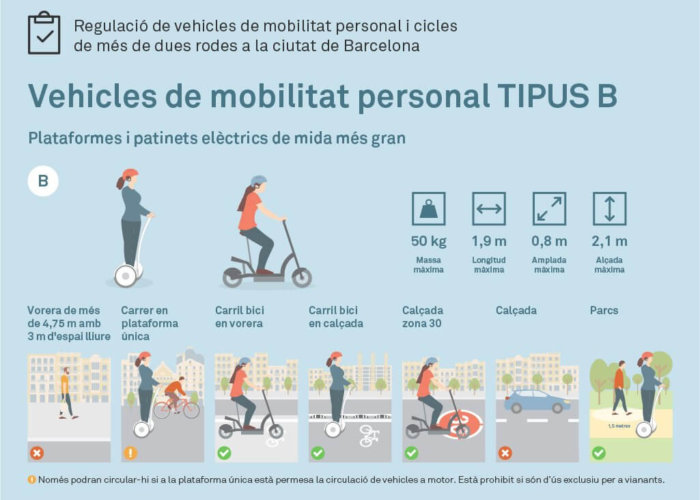
\includegraphics[width=12cm, height=7cm]{Marcteoric/normativaBCNpatinetselectrics.jpg}
    	\caption{Normativa de vehicles tipus B a Barcelona.}
\end{figure}

Si es parla de l'autonomia dels altres vehicles elèctrics no s'apropa ni de bon tros a l'autonomia d'un cotxe elèctric. Les autonomies d'aquests tipus de vehicles poden arribar als 40 minuts aproximadament, sent la bicicleta qui té una major autonomia. Depenent de la potència del motor, de la capacitat de la bateria i també com es condueixi aquest vehicle aquest temps pot variar. Un bon manteniment de la bateria també suposa una major durabilitat en l'autonomia. Ara es mostraran alguns vehicles elèctrics que són els que tenen un impacte més gran al mercat.

\subsection{Patinet elèctric}
%Patinets elèctrics
El patinet elèctric és una opció alternativa de transport ecològic per circular a nivell econòmic sense gastar res en gasolina. Són sustentables, lleugers, pràctics i ràpids. Són útils tant per aquelles persones amb mobilitat reduïda, com per estudiants, treballadors i persones amb l'objectiu de desplaçar-se d'una forma senzilla d'un lloc a un altre en un curt període de temps, estalviant gasolina i transport públic.

%Motor
L'enorme majoria dels patits tenen un motor anomenat Brush (amb escombretes de llarga durada), de gama econòmica. Els patinets elèctrics dissenyat per la conducció del peu, on el seu diàmetre de roda és més gran, disposen d'un altre gènere de motor anomenat Brushless, que vindria a fer el mateix que el motor Brush, però sense escombretes. \bigskip

%Autonomia 
L'autonomia del patinet elèctric és la combinació de múltiples factors: La capacitat de la bateria (Volts i Amperes), la potència del motor (Watts), càrrega del patinet elèctric (massa pròpia), càrrega (massa conductor), inclinació del terreny i velocitat.
En línies generals, un patinet elèctric acostuma a tenir una autonomia d'entre 40 minuts en models de 800W a 55-60 minuts en els models de 1000-1500W.
\bigskip

% Xiaomi Mi Scooter 
\subsubsection{Xiaomi Mi Scooter}  %Canviar mida per una més gran.
El Xiaomi Mi és el patinet elèctrics més venguts a la web d'Amazon. Està pensat per a una persona de fins a 75Kg. Té un abast de fins a 30Km amb una sola càrrega. Pot arribar a velocitats de fins a 35Km/h. El seu preu ronda els 380€. 
\begin{figure}[H]
		\centering
    	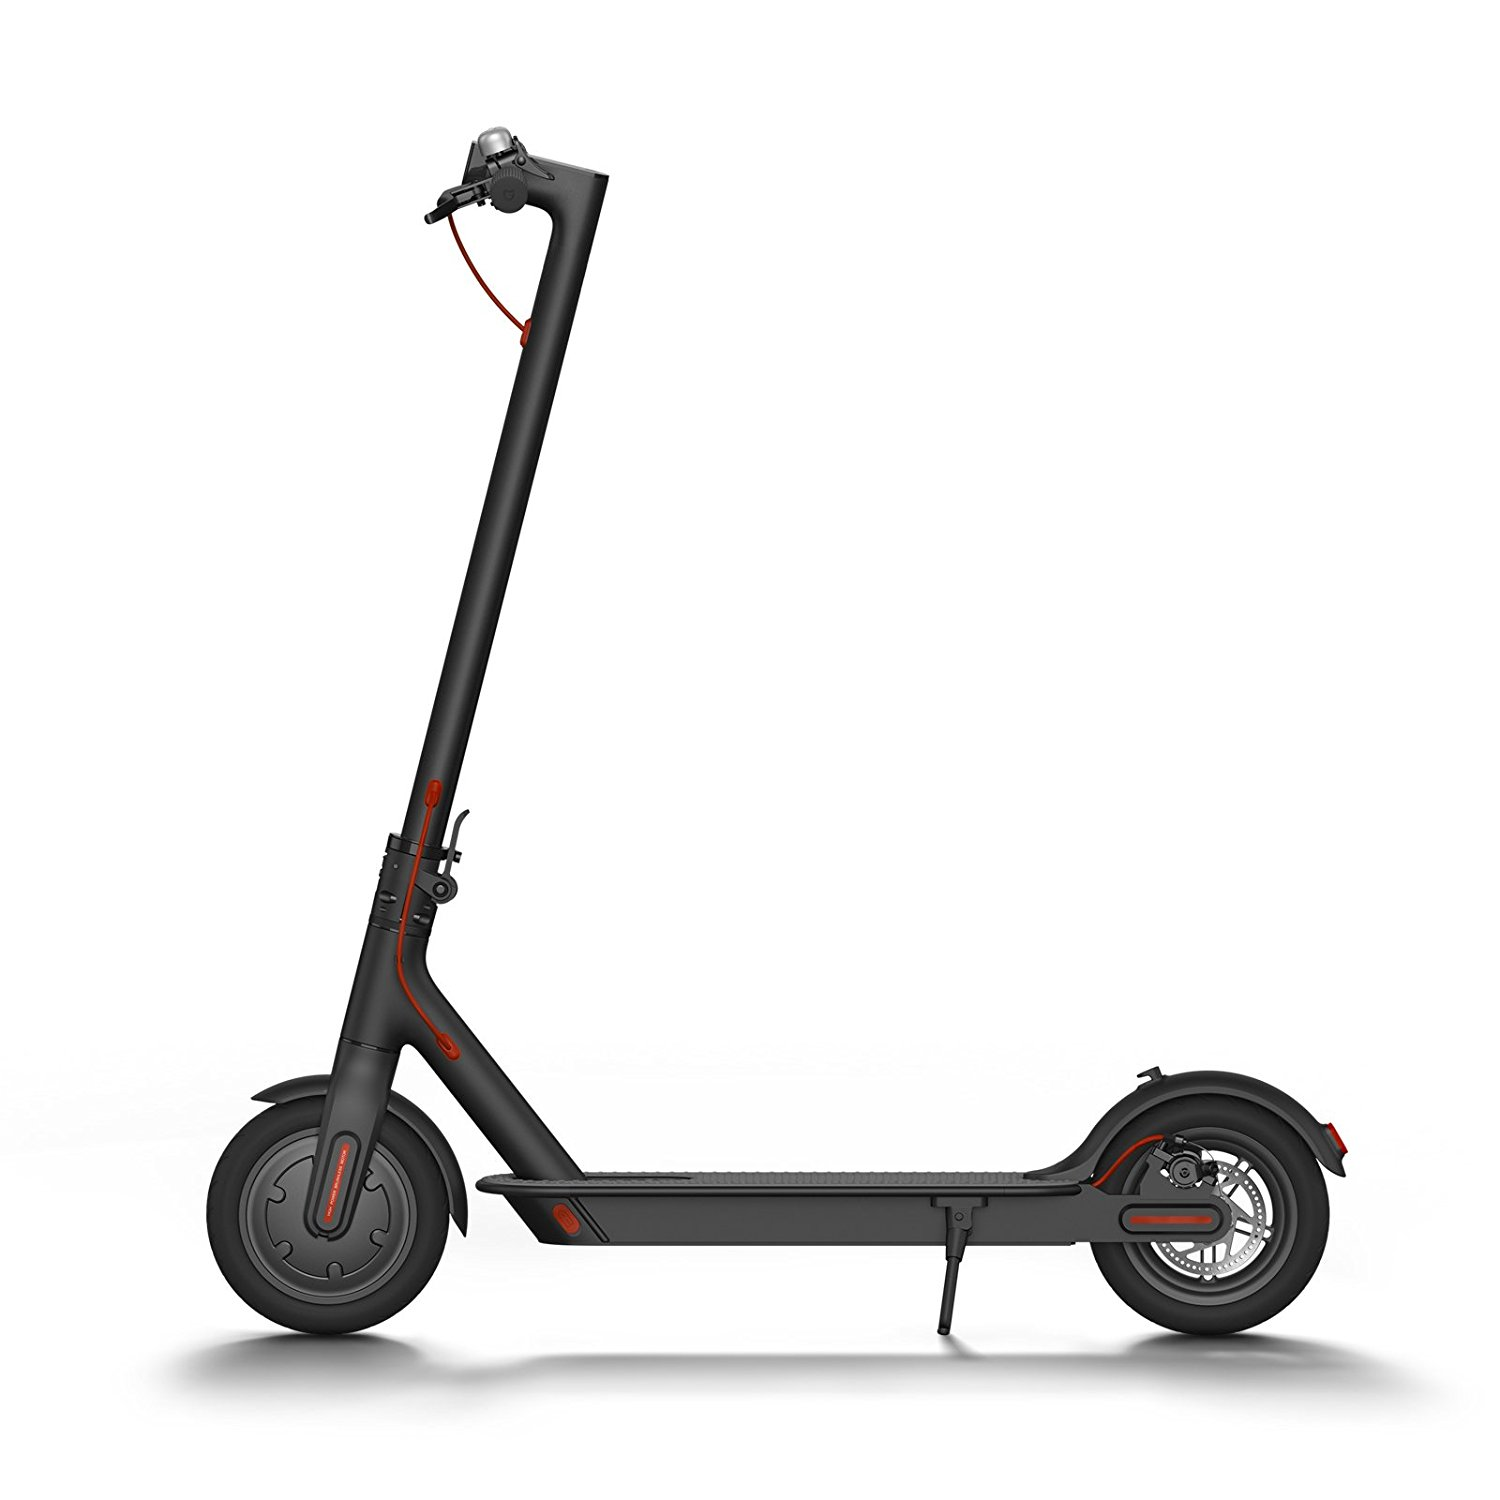
\includegraphics[width=10cm, height=10cm]{Marcteoric/patinetelectricxiamoi.jpg}
     	\caption{Xiaomi Mi Scooter.}
\end{figure}

\newpage

%Homcom Patinet elèctric
\textbf{Homcom Patinet elèctric} \bigskip \newline %Canviar per una mida més gran
El Homcom és un patinet plegable elèctric tipus Scooter, aquest model es trobaria a la gama baixa de patinets elèctrics. Està pensat per a una persona de fins a 50Kg. Té un abast d'entre 10-15Km amb una càrrega sencera. Pot arribar a una velocitat de fins a 12Km/h. El seu preu ronda els 100€.
\begin{figure}[H]
		\centering
    	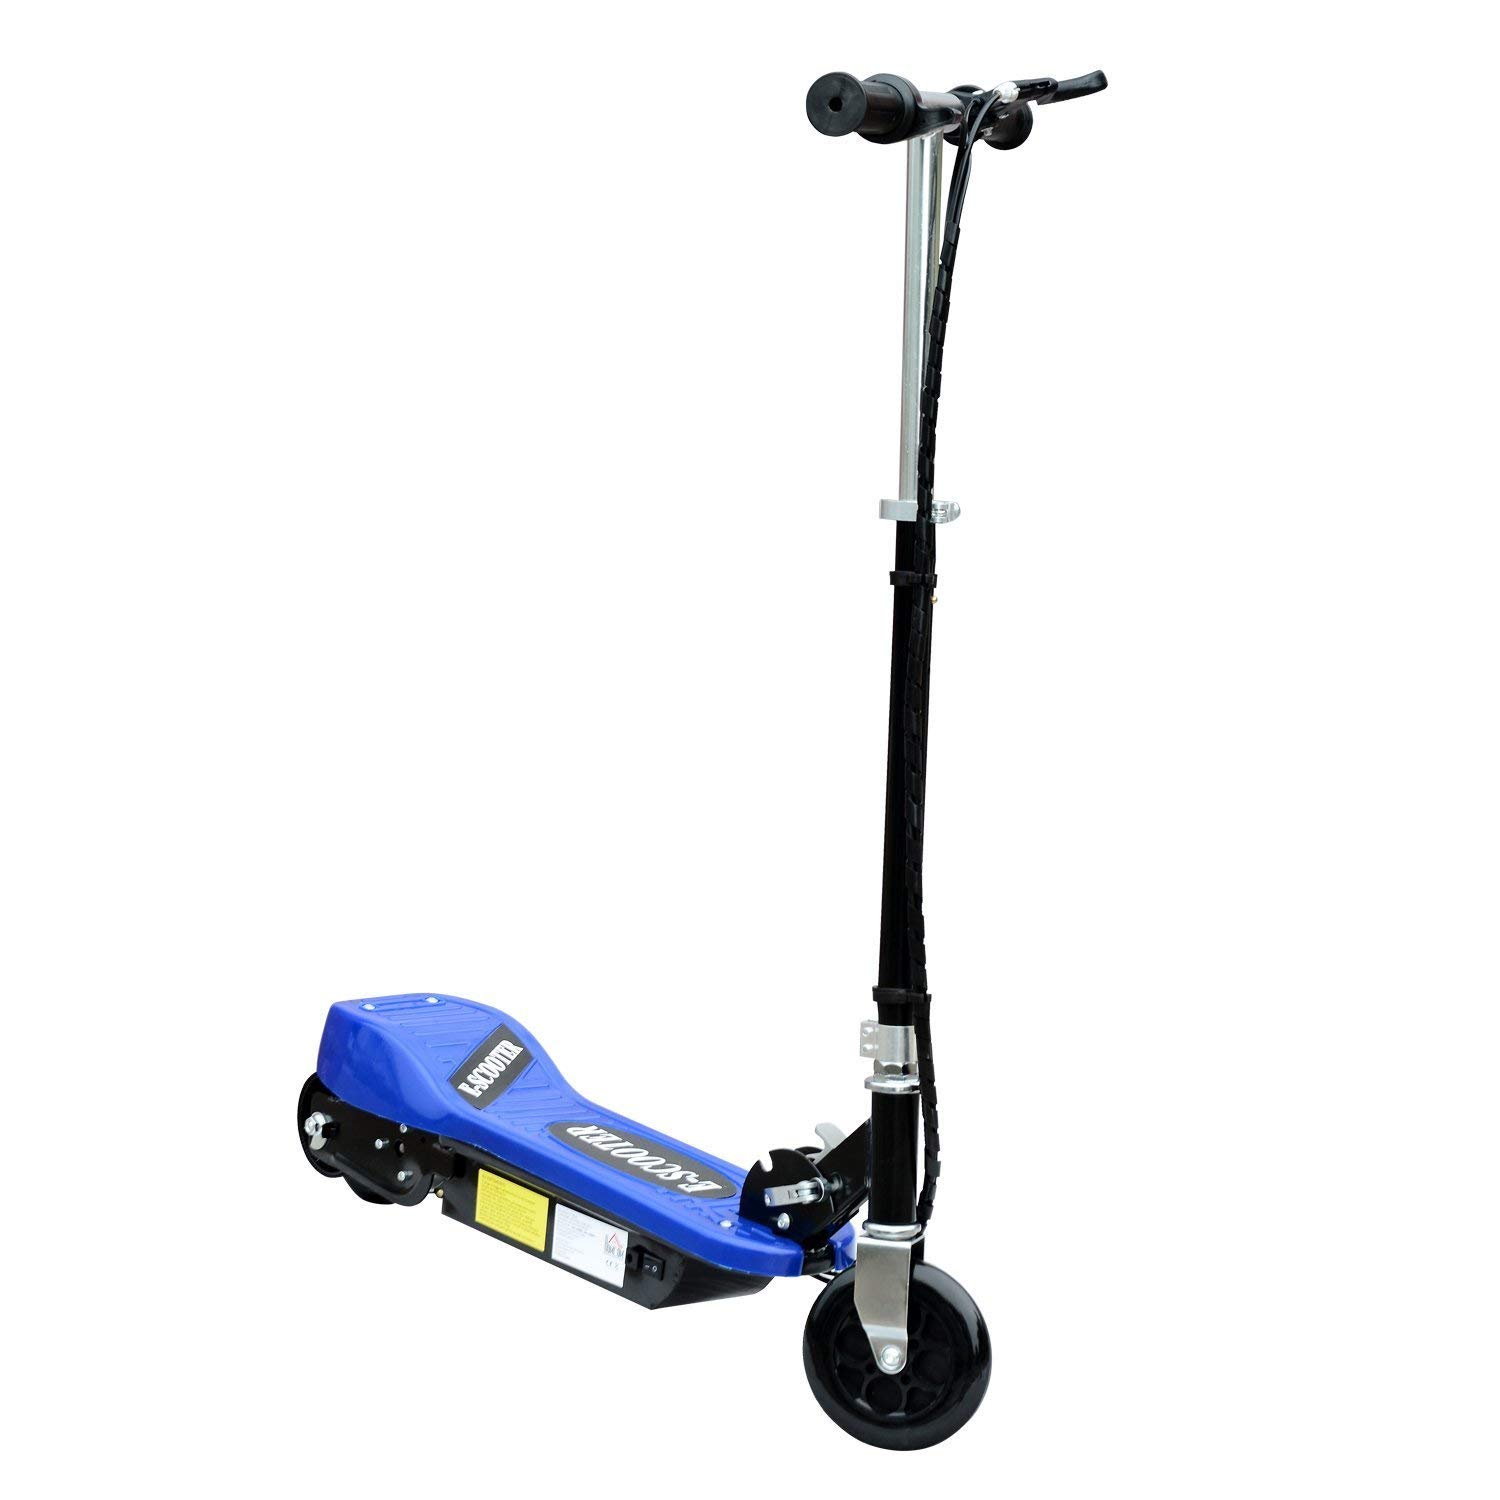
\includegraphics[width=8cm, height=8cm]{Marcteoric/Homcompatinetelectric.jpg}
     	\caption{Homcom patinet elèctric}
\end{figure}

%Hoverboard

\subsection{Hoverboard}
Aquests patinets han aparegut fa poc temps. Són únics en la forma en la que funcionen ja que s'autoequilibren, de tal forma que l'usuari pot accelerar i frenar tan sols movent el seu cos cap endavant o cap enrere. De la mateixa manera, girar és tan senzill com inclinar lleugerament el cos cap a un costat o l'altre. El funcionament d'aquest patinet es basa en el funcionament de diferents mecanismes. En primer lloc, les bateries es connecten a dos motors elèctrics independents en cada roda. Per altra banda, es troba el component més important per a mantenir l'equilibri, el giroscopi. Aquest detecta quan canvia d'orientació el patinet per a, d'aquesta forma, poder mantenir l'orientació adequada. 

El giroscopi funciona mitjançant un sensor magnètic que detecta la direcció de moviment i la velocitat rotacional de la roda. 
Tot el sistema es troba connectat a una unitat central de processament (CPU). El giroscopi mesura constantment l'orientació de la roda, i envia un senyal a la CPU per a que es processi e interpreti. D'aquesta forma, si el patinet s'inclina cap endavant s'envia l'ordre d'accelerar els motors per a compensar aquesta inclinació. Pel contrari, si s'inclina cap enrere es produirà l'efecte invers. Ara es mostraran dos exemples per veure com estan implantats aquests productes al mercat. \newline \bigskip

%Hooboard
\textbf{Hooboard} \bigskip \newline  
El Hooboard és un Hoverboard de gama alta. Té una autonomia de fins a 15Km i una velocitat màxima de fins a 15Km/h. Està composat per dos motors de 400W i el seu preu ronda els 500€.
\begin{figure}[H]
		\centering
    	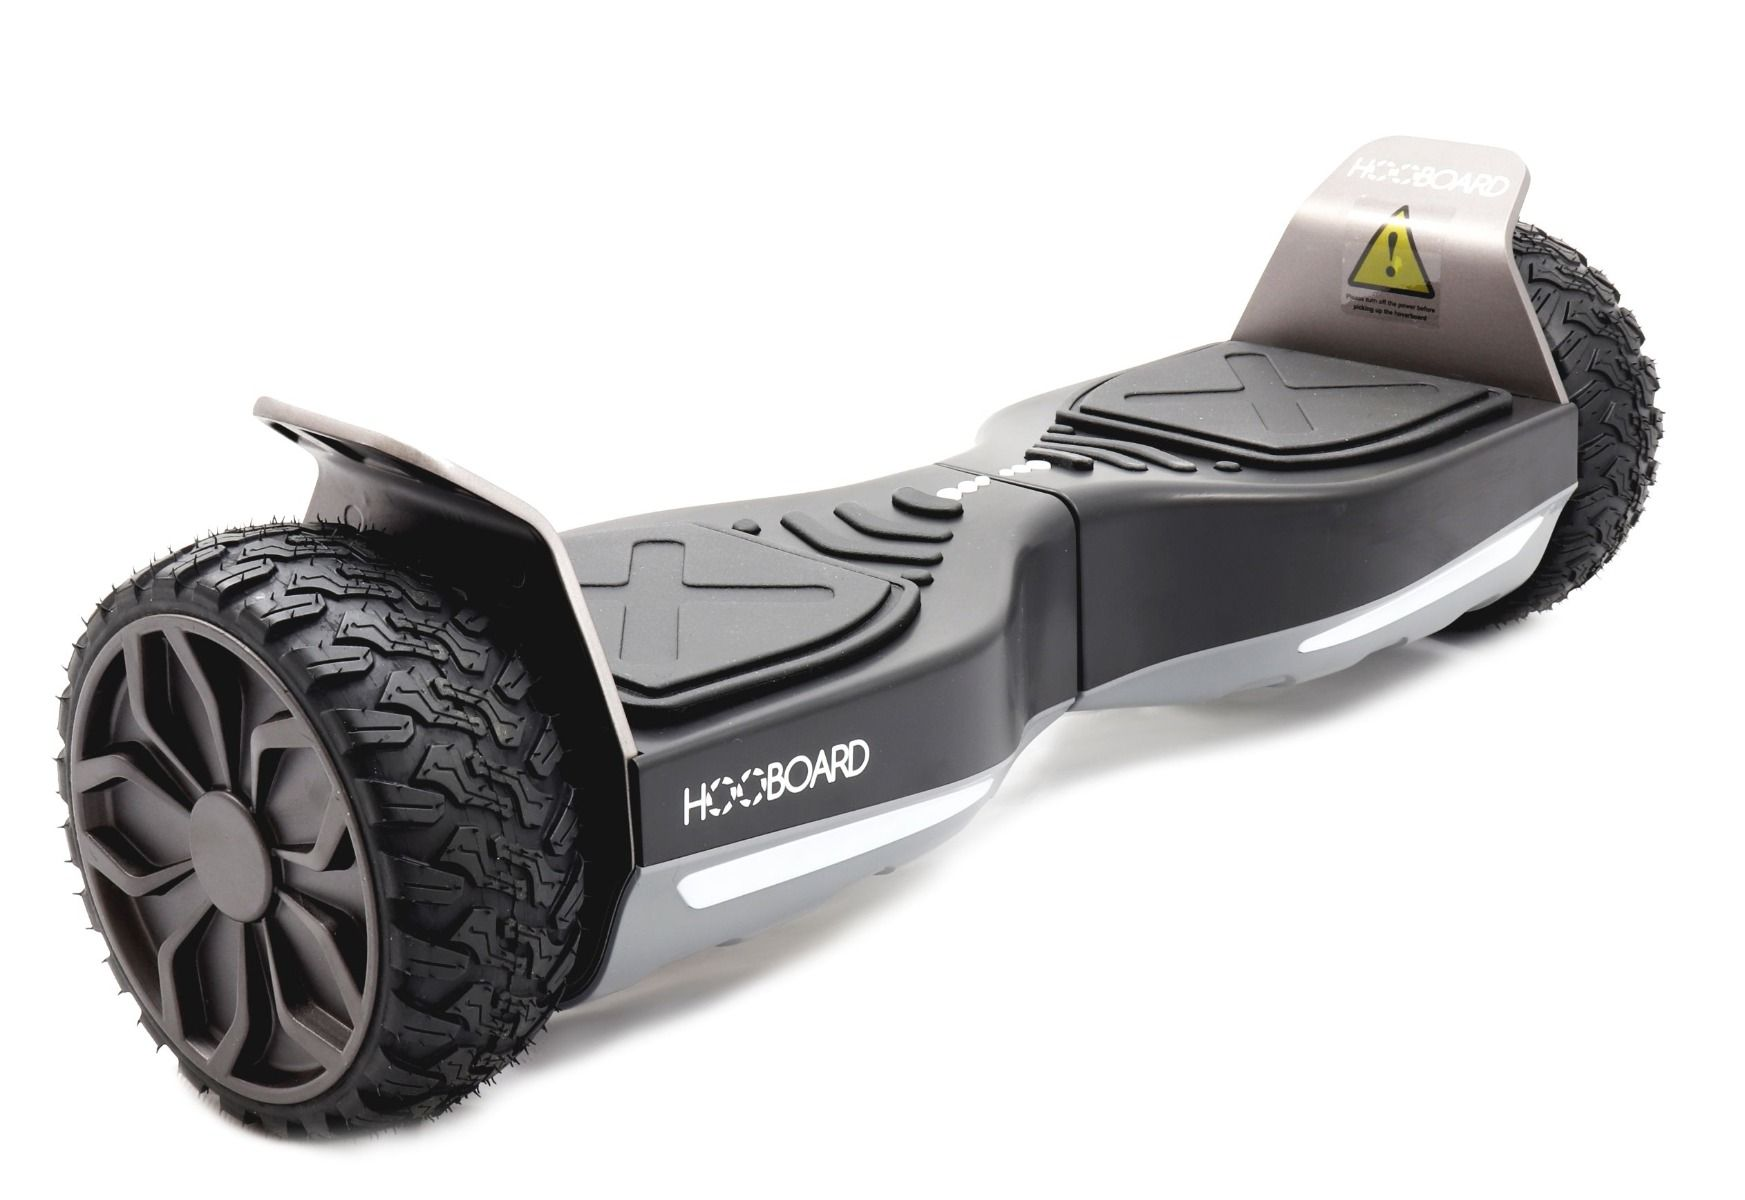
\includegraphics[width=9cm, height=7cm]{Marcteoric/hooboard.jpg}
     	\caption{Hooboard}
\end{figure}

\newpage

% BEBK Hooverboard
\textbf{BEBK Hooverboard} \bigskip  \newline % canviar per una mida més gran
El BEBK Hooverboard és un Hooverboard que funciona mitjançant motors elèctrics Brushless. Consta de dos motors de 350W. Pot arribar a velocitats de fins a 12Km/h i una autonomia de fins a 18Km. El seu preu ronda els 150€.
\begin{figure}[H]
		\centering
    	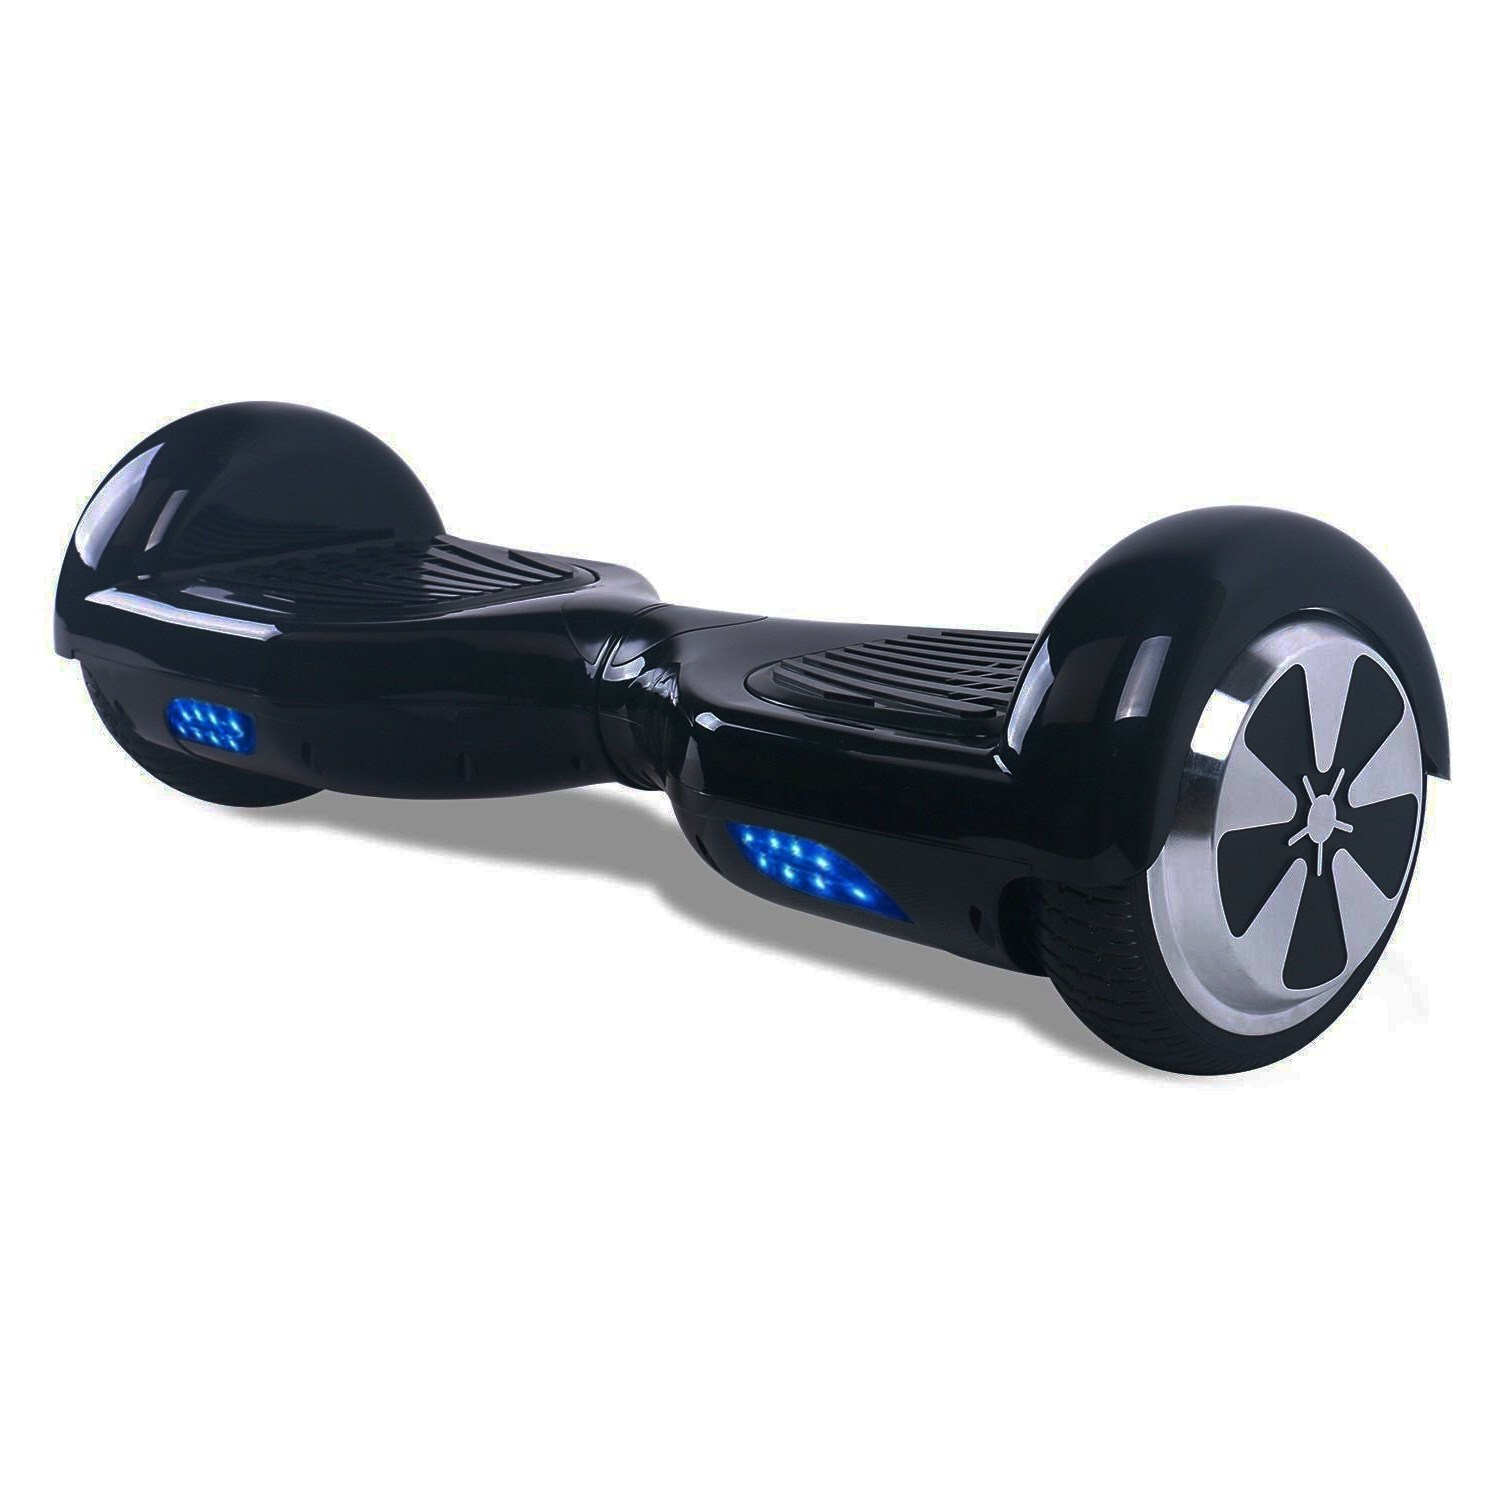
\includegraphics[width=7cm, height=7cm]{Marcteoric/bebkhooverboard.jpg}
     	\caption{BEBK Hooverboard}
\end{figure}

\subsection{Bicicleta elèctrica}
% Bicicletes elèctriques
Al 2016 les ventes de bicicletes elèctriques van arribar, en tot el món, a uns 35 milions d'unitats. La millora de la tecnologia de les bateries d'ions de liti està donant com a conseqüència bicicletes elèctriques més lleugeres, més econòmiques i cada cop més similars a les bicicletes tradicionals.

Les altes tasses d'urbanització, la millor de la tecnologia de les bateries i els components de les bicicletes, les polítiques locals relacionades amb la contaminació, el desig creixent d'abandonar modes de transport motoritzats, el seu major rendiment i baix cost impulsen la indústria de la bicicleta elèctrica. Les bicicletes elèctriques es troben situades en una posició ideal per a ser les majors beneficiades d'aquesta tendència de canvi, pel seu baix cost en relació amb l'automòbil, per no requerir carnet pel seu maneig i per l'existència, cada cop en major mesura d'infraestructures especialment dedicades a elles. \newline \bigskip

% Extrbici XF800 Electric ATV                 
\textbf{Extrbici XF800 Electric ATV } \bigskip	\newline	% canviar per una mida més gran
L'Extrbici XF800 Electric ATV és una bicicleta elèctrica que pot portar una càrrega de fins a 160Kg, pot arribar a 50Km/h amb una autonomia relativa de fins a 80Km. El seu preu rondaria els 1900€
\begin{figure}[H]
		\centering
    	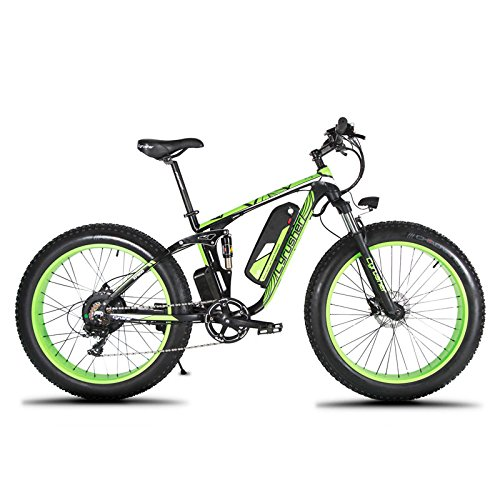
\includegraphics[width=10cm, height=10cm]{Marcteoric/extrbicixf800electricatv.jpg}
     	\caption{Extrbici XF800 Electric ATV}
\end{figure}
% FOLLOW UP E05                        
\textbf{FOLLOW UP E05 }	\bigskip \newline			% canviar per una mida més gran
El FOLLOW UP E05 és una bicicleta elèctrica que pot portar una càrrega de fins a 100Kg, pot arribar a 22Km/h amb una autonomia de fins a 30Km. Funciona amb motor Brushless de 250W i el seu preu ronda els 400€.
\begin{figure}[H]
		\centering
    	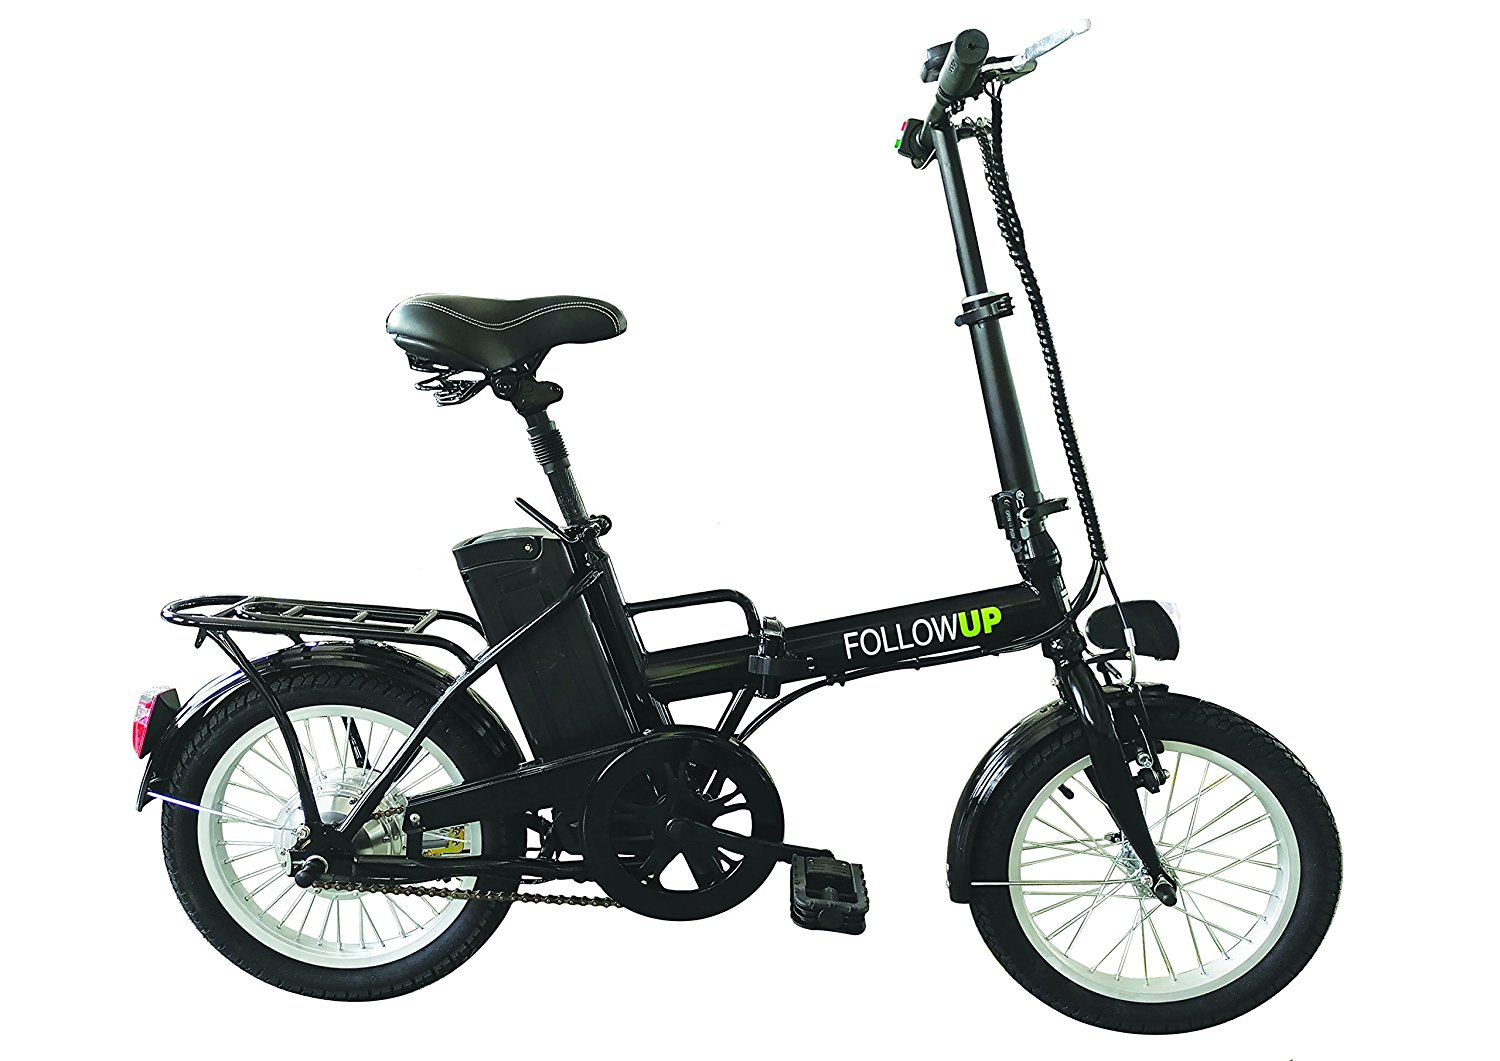
\includegraphics[width=10cm, height=7cm]{Marcteoric/followupe05.jpg}
     	\caption{Extrbici XF800 Electric ATV}
\end{figure}

%!!!!!!!!!!!!!!!!!!!!!!!!!!!!!!!!!!!!!!!!!!!!!!!!!!!!!!!!!!!!!!!!!!!!!!!!!!!!!!!!!!!!!!!!!!!!!!!!!!!!!!!!!!!!!!!!!!!!!!!!!!!!!!!!!!!!!!!!!!!!!!!!!!!!!!!!!!!!!!!!!!!!!!!!!!
% Conclusió total
%Aquests vehicles suposaran la facilitat de desplaçar-se d'una forma ràpida i còmode, ja que l'electricitat de la bateria serà qui s'encarregui de la transports ràpids no contaminants on les persones podran desplaçar-se 
%!!!!!!!!!!!!!!!!!!!!!!!!!!!!!!!!!!!!!!!!!!!!!!!!!!!!!!!!!!!!!!!!!!!!!!!!!!!!!!!!!!!!!!!!!!!!!!!!!!!!!!!!!!!!!!!!!!!!!!!!!!!!!!!!!!!!!!!!!!!!!!!!!!!!!!!!!!!!!!!!!!!!!!!!!!

\section {Mercat de les bateries emprades per als VE}

%Introducció
Les bateries d'ió-liti ja formen part de la vida quotidiana i estan incloses en telèfons mòbils, tauletes i raspalls de dents elèctrics, entre d'altres aplicacions. En els últims anys s'han produït diferents avenços tecnològics en aquest tipus de bateries per a poder ser emprades en els vehicles elèctrics. Encara que l'adopció dels vehicles elèctrics no estigui sent tan positiva com s'esperava, les bateries ja suposen un component cada cop més rellevant dins de la indústria automobilística. Donat que les bateries són una part significativa dels costos d'un vehicle elèctric, existeixen considerables incentius per augmentar l'eficiència dels seus processos de producció, reduir els seus costos i millorar el seu rendiment. El sistema elèctric es beneficiarà del desenvolupament d'aquestes bateries, al construir una solució per emmagatzemament de l'energia generada per les tecnologies renovables intermitents, que permetran reforçar la seva seguretat de subministrament.

Respecte als reptes que té aquesta tecnologia a superar, cal destacar la falta d'una única tecnologia d'emmagatzemament que sigui capaç de cobrir totes les necessitats del mercat. Això provocarà que el sistema pugui contemplar la incorporació de diferents tipus de bateries. 

\newpage 

Addicionalment, a l'igual que qualsevol altre component del sistema elèc- \newline tric, els sistemes de gestió de bateries hauran de lidiar amb els possibles atacs tecnològics que puguin sofrir. En definitiva, el desenvolupament dels vehicles elèctrics permetrà avançar en les tecnologies de bateries \newline d'emmagatzemament. Les bateries hauran de considerar-se com a part de l'estratègia de les energies renovables, contribuint a arribar a un sistema energètic més eficient.

\subsection{Previsió de mercat per al futur de les bateries}

Com ja s'ha comentat prèviament, les bateries jugaran un paper molt important dintre dels vehicles elèctrics. Això vol dir que ja s'implementen estratègies per tal d'optimitzar el màxim els costos i rendiment d'aquestes. A la dècada del 2030 podríem estar parlant que el preu de baixada respecte el 2010, que és quan van començar a aparèixer de forma global les bateries d'ió-liti estaria suposant aproximadament una reducció de cost de fins al 75\%. No només es reduiran els preus de les bateries, sinó que la compra \newline d'aquestes bateries augmentarà considerablement en els últims anys arribant a valors que superin els catorze mil milions de dòlars l'any 2026.
\begin{figure}[H]
		\centering
    	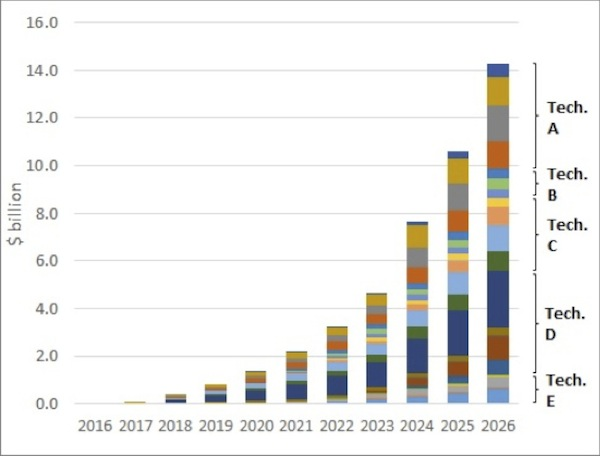
\includegraphics[width=13cm, height=8cm]{Marcteoric/ventabateries2026.jpg}
     	\caption{Previsió de ventes de bateries en funció del tipus de vehicle} 
\end{figure}

\subsection{L'hora de l'economia del liti}
Les bateries de liti estan totalment consolidades a la vida quotidiana. Són necessàries per alimentar des de petits dispositius fins a sofisticats vehicles elèctrics. La previsió és que el seu consum augmenti en els pròxims anys, especialment fomentat per l'auge de l'Internet de les Coses i altres aplicacions tecnològiques.

Degut a la predicció del decreixement del cost d'aquest tipus de bateries s'està impulsant de forma massiva aquest mercat. Aquesta caiguda de preus és probable que provingui d'un augment de la demanda degut a la propagació dels cotxes elèctrics, que està permetent als fabricants augmentar la producció. 
\begin{figure}[H]
		\centering
    	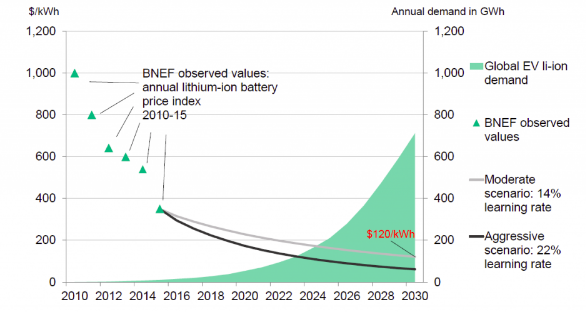
\includegraphics[width=13cm, height=8cm]{Marcteoric/mercatbaterialitioion.png}
     	\caption{Previsió del mercat de les bateries d'ions del liti.} 
\end{figure}

\subsection{Drivers de motors elèctrics}
% Drivers
%		Introducció
% 		Turnigy Dlux 250A 60V HV 14s ESC
% 		VESC 6 Complete - Vedder Electronic Speed Controller TRAMPA Exclusive
% 		Turnigy SK8-EXC V4.12 For Electric Skateboard Conversion w/BEC
% 		Controlador d'alta potència (Per buscar)	% DE MOMENT AQUEST L'IGNORO

% Introducció
Un sistema de control o controlador per a un motor elèctric podria definir-se com un dispositiu conjunt al motor, que serveix per governar d'alguna manera predeterminada l'operació del motor i que a més a més proporciona algun tipus de protecció que asseguri el seu funcionament. Els controladors poden ser molt senzills o extremadament complexes.\bigskip

avi en dia el motors predominats son els bruslles tan per aplkicacionde de hobby com veicels rc coma pets i mitgans veicles electris, per tan comentarem alguns dirnvers del marcat per tal de governar aquets motors per esmatar les sevas caracteristas i tenir una idea de quines magnituts es mouen els seus valors 
% !!!!!!!!!!!!!!!! AFEGIR ALGUNES COSETES MES COM A INTRODUCCIÓ?

\textbf{Turnigy Dlux 250A 60V HV 14s ESC}\bigskip \newline  
%Introducció del producte
Aquest ESC fa servir un disseny de PCB doble que separa l'alimentació del motor i del microcontrolador. Aquest disseny permet la disposició dels components òptims en cada PCB i proporciona la configuració ideal per la dissipació de calor i l'eficiència tèrmica. Ambdues PCB estan tancades en una carcassa d'alumini dissipador de calor per assegurar la dispersió de calor màxima. Las Fet de commutació en aquest CES són genuïnes de qualitat superior. El seu preu està al voltant dels 188€.
Tots els CES Turnigy Dlux es poden programar a través d'una tarjeta de programació o pel transmissor. \newline \bigskip 
% Especificacions
Especificacions:
	\begin{itemize}
            \item Intensitat continua màxima: 250A
            \item Max Burst actual: 275A
            \item BEC: N / A (OPTO)
            \item Lipo: 6 - 14S
            \item NiMH: 18 - 42 cel·les
            \item Pes: 456 grams
            \item RPM Max (2 pols): 200.000 rpm
            \item Mida: 135x77x50 mm
	\end{itemize}
% Característiques
Característiques:
	\begin{itemize}
			\item Baixa resistència interna
			\item Baixa temperatura de funcionament
			\item Protecció de sobreescalfament
			\item Eliminador d'espurnes
			\item Hexfets alta qualitat (MOSFETs)
	\end{itemize}
%Imatge
\begin{figure}[H]
		\centering
   	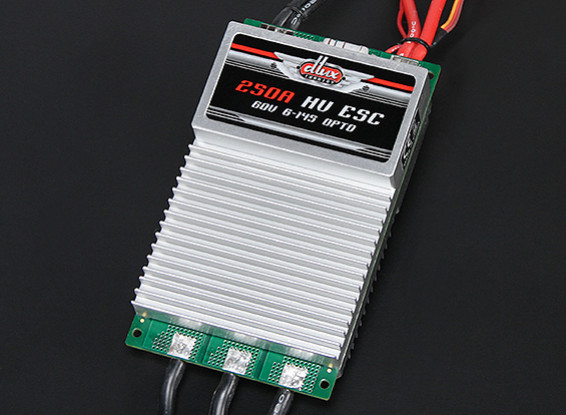
\includegraphics[width=8cm, height=8cm]{Marcteoric/250Hobydriver.jpg}
     	\caption{Turnigy Dlux 250A HV 14s ESC} 
\end{figure}
%Conclusions del producte        !!!!!!!!!!!!!!!A REVISAR
%Són controladors originalment dissenyats per controlar aparells RC, la seva potència pot perfectament ser emprada per a petits vehicles elèctrics. Dóna perfectament per moure patinets o bicicletes elèctriques. Funciona a 60V, per tant el voltatge de la bateria no seria molt perillós a l'hora de treballar-hi. Però li faltarien algunes funcions important com la frenada regenerativa i alguns controls d'arrencada progressiva i frenada que farien que l'autonomia i la comoditat de la conducció augmentés moltíssim. \bigskip

% VESC 6 Complete - Vedder Electronic Speed Controller TRAMPA Exclusive
% 		Introducció del producte	Per fer
% 		Especificacions				OK
% 		Característiques			OK
%		Imatge						OK
% 		Conclusions del producte	Per fer
\textbf{VESC 6 Complete - Vedder Electronic Speed Controller TRAMPA Exclusive}\smallskip
% Introducció del producte
 %!!!!!!!!!!!!!!!!!!!!!!!!!!!!!!!!!!!!!!!!!!!!!!!!!! PER FER
%\newline \bigskip 
% Especificacions
Especificacions:
\begin{itemize}
	\item Voltatge: 6V-60V (Segur per a 3S fins a 12S LiPO).
	\item Corrent: Continua 80A. Burst 120A. 
	\item 5V 1A de sortida per a electrònica externa.
	\item 3.3V 0.5A de sortida per a electrònica externa.
	\item Modes: DC, BLDC, FOC (sinusoïdal)
\end{itemize} 
% Característiques
Característiques:
\begin{itemize}
	\item Mesura de corrent i voltatge en totes les fases
	\item Frenada regenerativa
	\item Control de tracció (Simple i Parell)
	\item Sensored or Sensorless Operació + Mode híbrid
	\item Ports de comunicació: USB, CAN, UART
	\item Protecció ajustable per a definir els límits màxims i mínims \newline del voltatge i la corrent
\end{itemize}
% Imatge
\begin{figure}[H]
	\centering
	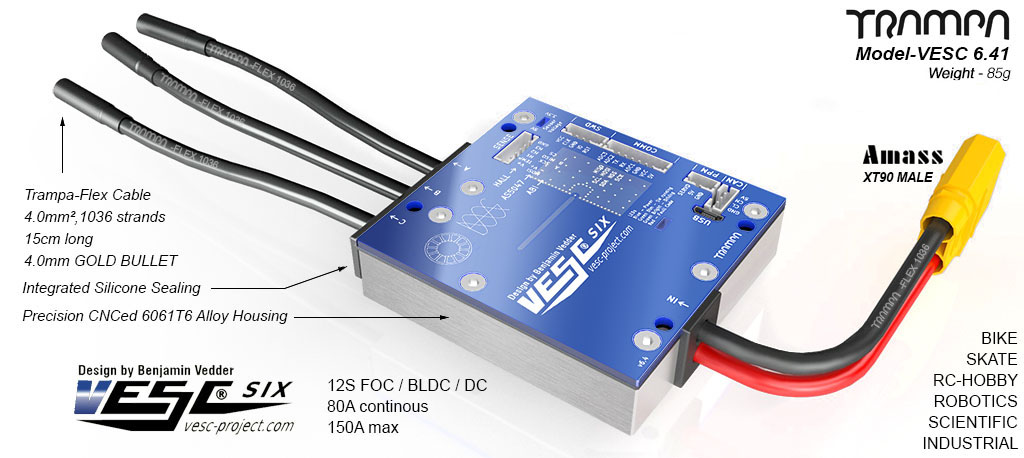
\includegraphics[width=\textwidth, height=8cm]{Marcteoric/drivertrampavesc6.jpg}
 	\caption{Turnigy Dlux 250A HV 14s ESC} 
\end{figure}

% Conclusions del producte
%!!!!!!!!!!!!!!!!!!!!!!!!!!!!!!!!! PER FER


% Turnigy SK8-EXC V4.12 For Electric Skateboard Conversion w/BEC
% 		Introducció del producte	Per fer
% 		Especificacions				OK
% 		Característiques			OK
%		Imatge						Per posar
% 		Conclusions del producte    Per fer

\textbf{Turnigy SK8-EXC V4.12 For Electric Skateboard Conversion w/BEC}

% Introducció del producte

% Especificacions
Especificacions: 	
\begin{itemize}
    \item Amperatge : 120A continu / 240A pic: 50A continu / 24            
	\item Cel·les: LiPo 3-12S
    \item Voltatge: 12.6 - 60V
    \item BEC 5V@1.5A
    \item Tipus BEC: Suport intern del controlador
    \item Timing: Calibratge Software
    \item Freqüència: PWM input
    \item Pes: 80gr
	\item Mides: 60x40x20mm
\end{itemize}

% Característiques
Característiques:
\begin{itemize}
	\item Frenada Regenerativa
	\item Sensored and Sensorless (FOC) permet que l'skate elèctric funcioni sense fer soroll el motor
	\item Seguretat: Control actual, funcions de control de temperatura
	\item Bona arrencada amb motors sensorless.
	\item Connectors de bala 12awg amb connector de bala de  4mm
\end{itemize}

% Conclusions del producte
%aqui etem parlant de dos controladors derivats del VESC un es una versio produda per sk8 del progecta obert o el vesc6 que es una versio millorada per una empresa privada derivan del que sera explicat mes endavent, tenan un sistema de aracada mes soua rampas i controlas de la frenada regenrativa i fan que la expariencia de conducio sigui mes amigable i eficas que amb un controlador de hoby 

%!!!!!!!!!!!!!!!!!!!!!!!!!!!!!!!!!!!!!!!!!!!!!!!!!!  DE MOMENT AQUEST L'IGNORO
% Controlador d'alta potència (Per buscar)
% 		Introducció del producte
% 		Especificacions
% 		Característiques
%		Preu
% 		Conclusions del producte

%\textbf{controladors comercial de alta potecia}\smallskip

% Introducció del producte
%http://www.sevcon.com/products/high-voltage-controllers/

% Especificacions
%Up to 800V DC peak supply voltage
%Up to 300kW peak power output
%Up to 150kW continuous power output

% Característiques

% Preu

% Conclusions del producte
%tambe tindriam una gama de controladors profecianls com el sevcon gen4-s10 que es un controlador disenyat per portar motors electrics desde  800V amb potencias de 150KW continus i pics de 300kw, tenen comunicacions amb can open per poder extreure o intruidir dadedes i els parametres de configuracio per tal de ferlos comportar com a EV o controladors indistrials. 


%!!!!!!!!!!!!!!!!!!!!!!!!!!!!!!!!!!!!!!!!!!!!!!!!!!!!!!!!!!!!!!!!!!!!!!!!!!!!!!!!!!!!!!!!!!!
% CONCLUSIONS TOTALS ?
%!!!!!!!!!!!!!!!!!!!!!!!!!!!!!!!!!!!!!!!!!!!!!!!!!!!!!!!!!!!!!!!!!!!!!!!!!!!!!!!!!!!!!!!!!!!

\section{Recerca de projectes de controladors de vehicles elèctrics de codi obert}
% BRUNET: POSA ALMENYS ELS LINKS DE POSSIBLES CONTROLADORS QUE PODRIEM COMPRAR AL MERCAT, ALMENYS NECESSITARIA UN PARELL D'ELLS, EL MODEL ECONOMIC I EL MODEL TOP DE GAMA. POSANT-ME EL LINK DEL PRODUCTE JA EM PODRIA ENCARREGAR JO D'OMPLIR TOT
% EVOLUCIÓ DEL MERCAT DELS CONTROLADORS
% EVOLUCIÓ DE LES TECNOLOGIES DELS CONTROLADORS EN UN FUTUR
% PACK TODO EN UNO
% DOS PACKS: BMS Y VESC


en al marcat actual tenin diversos controladors disponibles desde controlador de veicles de hoby i com coches o barcos RC fins a intermitgos i dedicats a pettis ev. tot tells tenan unas ventags i incovaniments derivats de la aplicacio en cuestio per que estan densenyats. esmatem les sevas caractaristiques: \bigskip

\textbf{HOBY:}\smallskip

son controladors original ment disenyats per controlar aparells de rc pero que la seva potecia pot perfectament ser utilisats en petits EV \smallskip

amb una potenica maximas de alguns models de 16.170w dona perfectament per poder moure patinets o bicicletes elecricas, el seu voltage baix 60 V  mes o menos, no seria molt parillos en estar en voltages vaixos, tenen el inconvaient que trevallan a gran intencitats i axo probo problemas se soroll i emis que san de tenir en conte tamde li faltan algunes funcions inportant com la frenada regenerativa i alguns control de arecada perogesia i frenada que farien que la autonima i la comoditat de cundocio aumantes moltisim. %\bigskip


\textbf{disaney per ev:}\smallskip

son controladors com alguns mdodels se sevcon o vesc entre molts altres, tenen potencias mes altesn el algun cas apar trevallaon a voltges molt mes alts, en el cuals san de tenir en conte, axo perment reduir la intenciat i disminir la secio del cables, disposne de control de frenada regentiva tan per rgenrar potencia o per cremar aquesta corrent contorl del ciquit de potencia

\textbf{controladors comercial de alta potecia}\smallskip

http://www.sevcon.com/products/high-voltage-controllers/

Up to 800V DC peak supply voltage
Up to 300kW peak power output
Up to 150kW continuous power output

tambe tindriam una gama de controladors profecianls com el sevcon gen4-s10 que es un controlador disenyat per portar motors electrics desde  800V amb potencias de 150KW continus i pics de 300kw, tenen comunicacions amb can open per poder extreure o intruidir dadedes i els parametres de configuracio per tal de ferlos comportar com a EV o controladors indistrials. 

% BRUNET: POSAR ALMENYS ELS LINKS DE POSSIBLES PROJECTES QUE PODRIEM TINDRE EN COMPTE PER A LA REALITZACIO DEL NOSTRE PROJECTE. JA AFIGIRIA TOTA LA XIXA.
% GITHUB: OPEN BMS
% GITHUB: VESC
% FALTARIA ALMENYS UN ALTRE I SI POGUESSIN SER UN TOTAL DE 3 PERFECTE.EN PLAN, UN DE BMS, UN DE VESC I UN DEL PACK. 

%Per fer una selecció de components en basem en 5V de baixa potencia com pot ser el VESC\footnote{http://vedder.se/2015/01/vesc-open-source-esc/} que es un dels controladors de EV mes emprats en el moment, l'objectiu no és millorar-ho sinó entendre el seu funcionament per dissenyar el nostre sistema més adaptat als nostres objectius. \smallskip
%per la part de control de bateryas en basem amb el progecte openBMS \footnote{https://github.com/rickygu/openBMS} 


%interasant https://upcommons.upc.edu/bitstream/handle/2117/108405/tfg-santiago-garci-a-sole-subido.pdf?sequence=1&isAllowed=y

\section{Marc del projecte}
% INDEX QUE EXPLIQUI COM DESENVOLUPARAS EL TEU PROJECTE AL LLARG DE LA DOCUMENTACIO.

per desebolupar el meu progrecte nesesitarem agafar informacio de com funcionan els motors electic i sobretot el bruslles ja que son els mes utilisats en aquestas aplicacions. una vagada tingem la informacio nanasaria per poder identificar con funcionan els motors bruslles i quin difrants tipus tenim anirem a buscar controladors del motor o ESC per tal de tenir una infocacio de com controlan aquets motors, analisam el funcionament dels controlaods comericals avera que trobem i si en tenim algun de obert per saver con funcionen quiens son la caractaristique i per a que son util en el cas que ens conve, 

